\chapter{Case study:\\PhaLP dataset}
To implement and evaluate hyperdimensional computing in real-life problems, the potential of hyperdimensional computing will be evaluated on the PhaLP dataset~\cite{phalp} for this chapter. PhaLP is a comprehensive database currently comprising more than 17000 entries of phage lytic proteins including much of their information such as their type, domains and tertiary structures. Phage lytic proteins are used by bacteriophages to infect bacterial cells. To cross the bacterial cell walls, phages use two different types of phage lytic proteins: virion-associated lysins (VALs) and endolysins. Phage lytic proteins also comprise one or more functional domains categorized into two classes: enzymatically active domains (EADs) and cell wall binding domains (CBDs).

All 17356 unique protein sequences were embedded into hyperdimensional vectors. This took only a few minutes for every method on a consumer laptop.

\section{Type classifcation}
Only a fraction of the database is manually annotated to include the protein's type because the amount of phage lytic proteins whose type is described in the literature is relatively small. The developers of PhaLP resorted to a machine learning approach for the classification of unannotated sequences. They embedded each protein sequence \textit{via} SeqVec~\cite{seqvec} and trained a random forest classifier with 100 estimators and balanced weights to classify the proteins whose types were unknown. For this case study, we attempted to simulate their experiments of classifying the proteins into types based on their sequence using several methods. As of March 2023, the latest version of the PhaLP database,~\textit{v2021\_04}, has been used to test our models.

First, we used several sequence encoding techniques tested on several kinds of base vectors. In chapter~\ref{ssec:protclas}, a method of embedding sequences of amino acids has already been discussed. Here, a sequence of amino acids is considered to be a bag of k-mers. Within a k-mer, the amino acids (presented as randomly generated hyperdimensional vectors) are bonded together with sequential information included. All possible k-mers are all then bundled together, the result is then a hyperdimensional vector representing the whole sequence. We also introduce a novel sequence embedding method within the framework of hyperdimensional computing. It is similar to the bag-of-words method in the sense that it bundles vectors of k-mers, but here, the k-mer's positional information will be encoded into the k-mer before bundling. The resulting sequences are then visually assessed \textit{via} PCA. 

There was no visual difference between the PCA plots for the bag-of-words method and the convolutional method, but there is a clear difference between the different starting embeddings. The sequence embeddings from both the bag-of-words method and the convolutional method made with ESM AA embeddings seem to capture more of the variance between the sequences. To demonstrate hyperdimensional computing as an option for machine learning applications, several methods using this framework have been developed and tested. Out of the 11549 unambiguous UniParc accessions in the newest version of the database, 4829 are manually annotated on their type. Out of these manually annotated proteins, 2803 are endolysins and 2026 are VALs.

\begin{figure}[H]
    \centering
    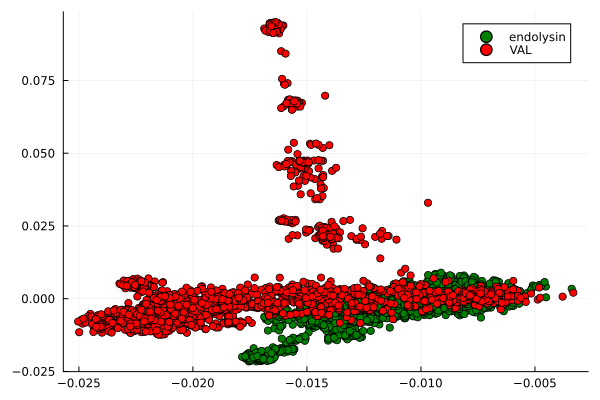
\includegraphics[scale = 0.5]{phalp_bow_rand}
    \caption{Scatter-plot of the first two principal components of the encoded phage lytic proteins. The sequences were encoded via the bag-of-words method starting from random hyperdimensional vectors. Only manually annotated phage lytic proteins were considered and are color-coded based on their type. These PCs account for roughly 7 \% of the total variance in the system.}
    \label{fig:phalpbowrand}
\end{figure}

\begin{figure}[H]
    \centering
    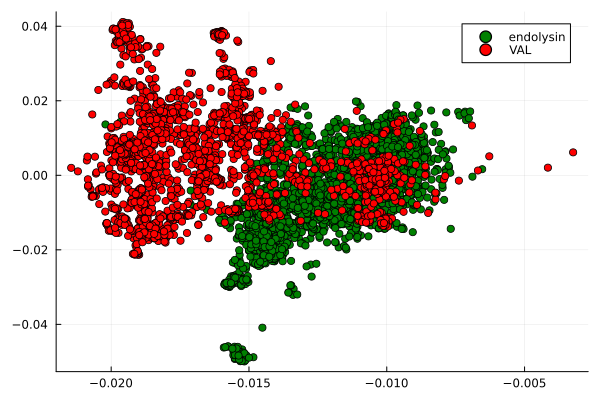
\includegraphics[scale = 0.5]{phalp_bow_esm}
    \caption{Scatter-plot of the first two principal components the encoded phage lytic protein. The sequences were encoded via the bag-of-words method starting from hyperdimensionally-extended ESM embeddings. Only manually annotated phage lytic proteins were considered and are color-coded based on their type. These PCs account for roughly 15.5 \% of the total variance in the system.}
    \label{fig:phalpbowesm}
\end{figure}

\subsection*{Purely hyperdimensional}\label{ssec:purehdc}
As a baseline level, we use the rudimentary HDV classification technique as seen in chapter~\ref{sec:example}: the HDVs of sequences of the same class are bundled to construct single HDVs representative of every class. Then, a sequence's class is inferred by comparing the sequence's HDV to both class HDV \textit{via} a similarity measure based on the assumption that the class vector is maximally similar to its components. This model was evaluated \textit{via} a stratified 10-fold cross validation.
\begin{table}[h]
    \caption{\label{tab:phalpclass}Results of type classifications using the principal classification technique of hyperdimensional computing and an XGBoost classifier with several kinds of embeddings}
    \resizebox{\textwidth}{!}{\begin{tabular}{|c||c|c|c|c|}
        \hline
        \underline{F1-scores} & \textbf{BoW random} & \textbf{BoW ESM} & \textbf{Convolutional random} & \textbf{Convolutional ESM} \\
        \hline
        \textbf{Purely HDC} & 0.1458 & 0.1468 & 0.1461 & 0.1461 \\
        \hline
        \textbf{XGBoost classifier} & 0.9667 & 0.9754 & 0.9661 & 0.986 \\
        \hline
    \end{tabular}}
\end{table}

It is feasible to learn the classes of every sequence using only operations within the hyperdimensional computing framework. This is done by using the same techniques as in chapter~\ref{sec:example}. Evaluating our model using stratified 10-fold cross-validation results in F1-scores of around 0.14 for every kind of hyperdimensional embedding. This low result is likely due to the possibility of oversaturation of the class vectors.

We can predict the angle between a class vector and a randomly selected vector from said class by $\Theta = \arccos({2k \choose k}/2^{2k})$ with $2k+1$ equal to the number of sequences in the class~\cite{sathdv}. This approximation is valid for binary or bipolar vectors in hyperdimensions $(\ge 10000)$. This equation also suggests that an increase in dimensions will not influence the angle. Evaluating this equation by considering random 1001 vectors in a class, so $k = 500$, results in an angle of $88.6^{\circ}$. This indicates that a vector has a limited capacity: the more vectors we bundle together, the closer the angle will be to $90^{\circ}$ and thus the more dissimilar the class vector becomes to its components. This equation assumes that the class vector is a bundle of purely random vectors which is not the case for our embeddings; however, it provides us a rough idea about the bundling capacity of a hyperdimensional vector. Thus, using the rudimentary model works only for very small datasets, like seen in the examples in chapter \ref{sec:example}. To encode larger datasets, the training algorithm has to be more refined.

\subsection*{Machine learning models with binary hyperdimensional embeddings}
The baseline hyperdimensional classifcation model has been compared to a more established model, the XGBoost classifier. The classification with an XGBoost classifier is done via the default XGBoost classifier from \textit{XGBoost.jl v2.2.5} and is evaluated \textit{via} \textit{MLJ.jl v0.19.5} with also a stratified 10-fold cross validation. The results for every embedding with this model are much more comparable to the results of the experiment in the PhaLP paper. This is an indication that hyperdimensional computing can provide a very fast and reliable method of embedding protein sequences, even without prior biological information.